\chapter{Szimulációk}
A teljes struktúrát együttesen nem szimuláltam le, mivel az egyes alkotóelemek méretezését külön-külön végeztem első körben, de még nem minddel jutottam értékelhető eredményre. A differenciális vonallal és az antennával sikerült teljesítenem a követelményeket, a balun és a földkitöltés szélén az áramblokkoló mintázat még nincs használható állapotban.
\section{A balun transzformátor}
\par Az balunnal jelenlegi konstrukciójával egyszerűen nem teljesült a maximum -10 dB-s bemeneti (CPW) reflexiós követelmény a kimenet (CPS) illesztett lezárása mellett. Az áramblokkoló mintázat tervezésével pedig azért nem foglalkoztam, mert ennek a vizsgálatához érdemes a többi komponenst elfogadhatóan megtervezni, mivel ez a mintázat gyakorlatilag csak az antenna sugárzási karakterisztikáját kell, hogy befolyásolja. Ugyan a földkitöltés viselkedése az antenna bemeneti impedanciáját is kissé megváltoztathatja, de tapasztalataim szerint csak olyan mértékben, hogy az az antenna paramétereinek enyhe változtatásával az újból kihangolható.
\par A legjobb szimulált balun bemeneti reflexió \aref{fig:balun-s11}. ábrán látható, a szimulációhoz a balun keresztmetszetei \aref{fig:balun-kereszt}. ábrán, a balun méretparaméterei pedig \aref{tab:balun-param}. táblázatban láthatóak. A bemeneti reflexióra adódó értékekre általánosan igaz volt, hogy a vizsgált frekvenciasávban alig változott, gyakorlatilag konstans volt, így a balunnak nem a sávszélessége a korlátozó tényezője, legalább erre a struktúrára.
\begin{figure}[h]
	\centering
	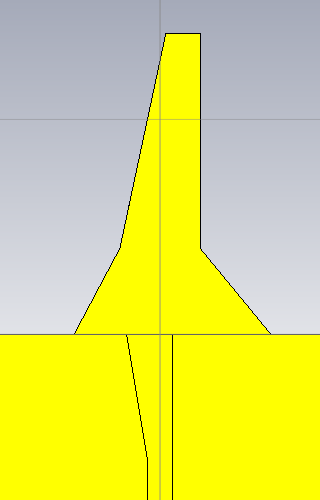
\includegraphics[width=0.3\textwidth]{kep/results/balun_1.png}
	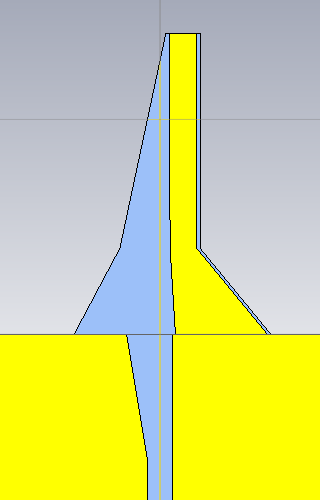
\includegraphics[width=0.3\textwidth]{kep/results/balun_2.png}
	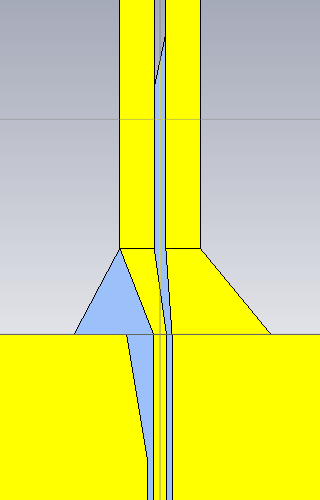
\includegraphics[width=0.3\textwidth]{kep/results/balun_3.png}
	\caption{A szimulált balun struktúra keresztmetszetei.}
	\label{fig:balun-kereszt}
\end{figure}
\begin{figure}[h]
	\centering
	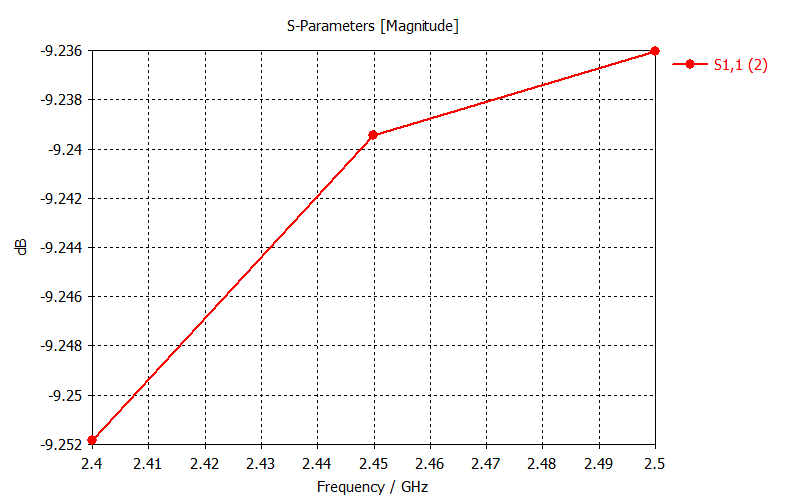
\includegraphics[width=0.8\textwidth]{kep/results/balun_S11.png}
	\caption{A magában álló, illesztetten lezárt balun szimulált bemeneti reflexiója.}
	\label{fig:balun-s11}
\end{figure}
\begin{table}[h!]
	\centering
	\begin{tabular}{||c|c|c|c|c|c|c|c||}
	\hline\hline
	$a_{asd}$ & $b_{asd}$ & $c_{asd}$ & $d_{asd}$ & $e_{asd}$ & $f_{asd}$ & $g_{asd}$ & $h_{asd}$ \\ 
	\hline
	\SI{1,55}{mm} & \SI{1,55}{mm} & \SI{0,03}{mm} & \SI{0,274}{mm} & \SI{0,8}{mm} & \SI{100,19}{\ohm} & \SI{74,4}{\ohm} & \SI{74,4}{\ohm}\\
	\hline\hline
	$a_{asd}$ & $b_{asd}$ & $c_{asd}$ & $d_{asd}$ & $e_{asd}$ & $f_{asd}$ & $g_{asd}$ & $h_{asd}$ \\
	\hline
	\SI{1,55}{mm} & \SI{1,55}{mm} & \SI{0,03}{mm} & \SI{0,274}{mm} & \SI{0,8}{mm} & \SI{100,19}{\ohm} & \SI{74,4}{\ohm} & \SI{74,4}{\ohm}\\
	\hline\hline
	\end{tabular}
	\caption{asd}
	\label{tab:balun-param}
\end{table}